% abtex2-modelo-artigo.tex, v-1.9.2 laurocesar
% Copyright 2012-2014 by abnTeX2 group at http://abntex2.googlecode.com/ 
%

% ------------------------------------------------------------------------
% ------------------------------------------------------------------------
% abnTeX2: Modelo de Artigo Acadêmico em conformidade com
% ABNT NBR 6022:2003: Informação e documentação - Artigo em publicação 
% periódica científica impressa - Apresentação
% ------------------------------------------------------------------------
% ------------------------------------------------------------------------

\documentclass[
	% -- opções da classe memoir --
	article,			% indica que é um artigo acadêmico
	11pt,				% tamanho da fonte
	oneside,			% para impressão apenas no verso. Oposto a twoside
	a4paper,			% tamanho do papel. 
	% -- opções da classe abntex2 --
	%chapter=TITLE,		% títulos de capítulos convertidos em letras maiúsculas
	%section=TITLE,		% títulos de seções convertidos em letras maiúsculas
	%subsection=TITLE,	% títulos de subseções convertidos em letras maiúsculas
	%subsubsection=TITLE % títulos de subsubseções convertidos em letras maiúsculas
	% -- opções do pacote babel --
	english,			% idioma adicional para hifenização
	brazil,				% o último idioma é o principal do documento
	sumario=tradicional
	]{abntex2}


% ---
% PACOTES
% ---

% ---
% Pacotes fundamentais 
% ---
\usepackage{lmodern}			% Usa a fonte Latin Modern
\usepackage[T1]{fontenc}		% Selecao de codigos de fonte.
\usepackage[utf8]{inputenc}		% Codificacao do documento (conversão automática dos acentos)
\usepackage{indentfirst}		% Indenta o primeiro parágrafo de cada seção.
\usepackage{nomencl} 			% Lista de simbolos
\usepackage{color}				% Controle das cores
\usepackage{graphicx}			% Inclusão de gráficos
\usepackage{microtype} 			% para melhorias de justificação
% ---
		
% ---
% Pacotes adicionais, usados apenas no âmbito do Modelo Canônico do abnteX2
% ---
\usepackage{lipsum}				% para geração de dummy text
\usepackage{float} % para usar H em tabelas e figuras
\usepackage{listings} % para usar código fonte
\usepackage{xcolor} % para colorir o código fonte
% ---
		
% ---
% Pacotes de citações
% ---
\usepackage[brazilian,hyperpageref]{backref}	 % Paginas com as citações na bibl
\usepackage[alf]{abntex2cite}	% Citações padrão ABNT
% ---

% Custom style configuration for code layout
\lstset{
    frame=tb,                           % Frames the code top and bottom
    language=Python,                     % Set your default programming language
    aboveskip=3mm,
    belowskip=3mm,
    showstringspaces=false,
    columns=flexible,
    basicstyle={\small\ttfamily},
    keywordstyle=\color{blue},
    commentstyle=\color{gray},
    stringstyle=\color{purple},
    breaklines=true,                    % Automatically wrap long lines
    breakatwhitespace=true,
    tabsize=4
}
% ---
% Configurações do pacote backref
% Usado sem a opção hyperpageref de backref
\renewcommand{\backrefpagesname}{Citado na(s) página(s):~}
% Texto padrão antes do número das páginas
\renewcommand{\backref}{}
% Define os textos da citação
\renewcommand*{\backrefalt}[4]{
	\ifcase #1 %
		Nenhuma citação no texto.%
	\or
		Citado na página #2.%
	\else
		Citado #1 vezes nas páginas #2.%
	\fi}%
% ---

% ---
% Informações de dados para CAPA e FOLHA DE ROSTO
% ---
\titulo{Processamento de Alto Desempenho\\ Relatório Aula Prática}
\autor{Matesu Hashimoto}
\local{Brasil}
\data{2026, Taubaté}
% ---

% ---
% Configurações de aparência do PDF final

% alterando o aspecto da cor azul
\definecolor{blue}{RGB}{41,5,195}

% informações do PDF
\makeatletter
\hypersetup{
     	%pagebackref=true,
		pdftitle={\@title}, 
		pdfauthor={\@author},
    	pdfsubject={Paralelismo},
	    pdfcreator={pdflatex with abnTeX2},
		pdfkeywords={Computacao}{Paralelismo}{Unitau}{Relatorio}{artigo científico}, 
		colorlinks=true,       		% false: boxed links; true: colored links
    	linkcolor=blue,          	% color of internal links
    	citecolor=blue,        		% color of links to bibliography
    	filecolor=magenta,      		% color of file links
		urlcolor=blue,
		bookmarksdepth=4
}
\makeatother
% --- 

% ---
% compila o indice
% ---
\makeindex
% ---

% ---
% Altera as margens padrões
% ---
\setlrmarginsandblock{3cm}{3cm}{*}
\setulmarginsandblock{3cm}{3cm}{*}
\checkandfixthelayout
% ---

% --- 
% Espaçamentos entre linhas e parágrafos 
% --- 

% O tamanho do parágrafo é dado por:
\setlength{\parindent}{1.3cm}

% Controle do espaçamento entre um parágrafo e outro:
\setlength{\parskip}{0.2cm}  % tente também \onelineskip

% Espaçamento simples
\SingleSpacing


 % Carrega informações de dados para CAPA e FOLHA DE ROSTO

% ----
% Início do documento
% ----
\begin{document}

% Retira espaço extra obsoleto entre as frases.
\frenchspacing 

% ----------------------------------------------------------
% ELEMENTOS PRÉ-TEXTUAIS
% ----------------------------------------------------------

%---
%
% Se desejar escrever o artigo em duas colunas, descomente a linha abaixo
% e a linha com o texto ``FIM DE ARTIGO EM DUAS COLUNAS''.
% \twocolumn[    		% INICIO DE ARTIGO EM DUAS COLUNAS
%
%---
% página de titulo
\maketitle
\begin{resumoumacoluna}
O presente relatório se dispõe a discutir a implementação dos programas de paralelismo com o objetivo de resolver os problemas apresentados pela Lista de exercícios. Cada capítulo representa um dos problemas propostos, onde se é discutida a estratégia de implementação, quais operações MPI foram utilizadas e a sua validação. A seguir é apresentada uma análise de desempenho, através do uso de métricas de speed-up e eficiência, demonstrando as limitações da paralelização e concluindo se a utilização do MPI é vantajosa.


 \vspace{\onelineskip}
 
 \noindent
 \textbf{Palavras-chaves}: paralelismo. mpi. processamento de alto desempenho.
\end{resumoumacoluna}

% ]  				% FIM DE ARTIGO EM DUAS COLUNAS
% ---

% ----------------------------------------------------------
% ELEMENTOS TEXTUAIS
% ----------------------------------------------------------
\textual

% ----------------------------------------------------------
% Problemas
% ----------------------------------------------------------
\section{Problema 1 - Estatísticas}
Trata-se de um problema simples de se somar N valores e calcular sua média. Nesse caso N foi decomposto em um array de dados utilizando-se np.array\_split da biblioteca \citeonline{numpydoc}, pois pode-se usar um N não divisível por size. O retorno da função é N\%size sub-arrays de tamanho N//size + 1 e o resto(dos subarrays) de tamanho N//size. 

Para -se calcular a média, deve se atentar para calcular a média das médias de cada bloco pois os tamanho dos dados locais difere. Se eles fossem de tamanhos iguais $(N\_rank0 = N\_rank1 = ... = N\_rankN)$ então poderia-se usar reduce para somar as médias.
Para se calcular corretamente a média global deve-se usar reduce na soma de cada array de dados local e o tamanho desse array. 

A validação foi realizada se comparando com as funções np.sum e np.mean do numpy e nesse exercício não se fez comparações de Desempenho, logo não se pode afirmar que a paralelização é vantajosa ou não(provavelmente é).

\section{Problema 2: Gather Reduce}
O problema se dispõe a comparar o tempo de execução do gather e do reduce com processos de 1, 2, 4 e 8. Abaixo segue a tabela com os tempos de execução de cada um dos métodos:

\begin{table}[H]
\centering
\begin{tabular}{|c|c|c|}
\hline
\textbf{Processos} & \textbf{Gather (s)} & \textbf{Reduce (s)} \\ \hline
1 & 0.15328741300027104 & 0.15738252000028297 \\ \hline
2 & 0.1735095040003216  & 0.18257671099991057\\ \hline
4 & 0.16784756300012305 & 0.14800468299972636 \\ \hline
8 & 0.15755982599966956 & 0.1503943029997572 \\ \hline
\end{tabular}
\caption{Tempos de execução do gather e reduce}
\label{tab:tempos}
\end{table}

Pela tabela acima, pode-se notar que os resultados são praticamente iguais, com a maior diferença de tempo sendo de aproximadamente 0.02 segundos(linha 2). 
Como há uma equivalência de resultados, o método reduce possui uma vantagem que é a de não precisar de código adicional para processar os resultados individuais além de não precisar transferir mais informações para o processo root. 

Com isso, o reduce é mais adequado para problemas grandes, visto que o nó raiz só recebe o resultado final, sem precisar armazenar individualmente cada resultado. 

\section{Problema 3 - Integração Numérica}
O problema requer que se faça a integração da função $f(x) = sin(x)$ no intervalo $[0, \pi]$ usando o método do ponto médio. A função é integrada numericamente usando a regra do ponto médio, que é uma técnica de integração numérica que aproxima a integral de uma função usando retângulos. O intervalo de integração é dividido em subintervalos, e a altura de cada retângulo é determinada pelo valor da função no ponto médio de cada subintervalo.

Para isso o valor de N utilizado foi de 100.000.000 subretângulos, onde cada processo ficou responsável por calcular localmente os índices que pertencem ao seu intervalo e consequentemente realizar a soma local que por fim foi reduzida para o processo 0 em uma soma global. 

Para não se utilizar o scatter(e ter que transferir 100.000.000 valores entre os processos) usou-se for i in range(rank, N, size) que define localmente os indice como no exemplo de -n 4 e N = 100:

rank 0:
  for i in range(0, 100, 4) -> 0 4 8 12 ... 

rank 1:
  for i in range(1, 100, 4) -> 1 5 9 13 ...

rank 2: 
  for i in range(2, 100, 4) -> 2 6 10 14 ...

rank 3:
  for i in range(3, 100, 4) -> 3 7 11 15 ...

Esse método é uma decomposição cíclica dos dados.

Na estratégia de solução, apenas a, b e N são transmitidos por broadcast, passando apenas 3 valores em vez de N//size valores por rank. 

\section{Problema 4 - Estimativa de $\pi$ pelo Método de Monte Carlo}
O problema gera aleatoriamente e localmente um conjunto de pontos entre $-1 <= 1$ de tamanho $N//size$ e calcula localmente quais desses pontos estão dentro do círculo e através de dois reduces calcula o total de pontos dentro do círculo e o total de pontos gerados. O processo root então faz a estimativa de $\pi$ através da fórmula: 

\begin{equation}
  pi = 4*\frac{total\_dentro\_circulo}{total\_gerado}
\end{equation}

O programa gerou a seguinte tabela de resultados:
\begin{table}[H]
\centering
\begin{tabular}{|c|c|c|}
\hline
\textbf{Processos} & \textbf{Estimativa} & \textbf{Tempo Execução} \\ \hline
1 & 3.14160792 & 28.35727361399995 \\ \hline
2 & 3.14164428  & 14.7583513579998\\ \hline
4 & 3.14189552 & 7.9102041789999475 \\ \hline
8 & 3.1419221656768865 & 6.13996790300007 \\ \hline
\end{tabular}
\caption{Tempos de execução e estimativa de $\pi$}
\label{tab:pi}
\end{table}

Se todos os processos utilizassem o mesmo vetor de pontos[N//size, N//size] definido fixo, a estimativa de $\pi$ seria a mesma para todos os processos. No entanto, como cada processo gera aleatoriamente seus próprios pontos, a estimativa de $\pi$ pode variar entre execuções diferentes.

Se os pontos[N, N] fossem um vetor definido fixo como na implementação linear, precisaria usar o scatter para passar para os outros processos, na implementação utilizada o vetor foi definido com valores aleatórios para não se haver a necessidade de comunicar os dados entre o rank 0 e os demais ranks.

Gerar localmente é melhor para um gerenciamento de memória pois assim o rank 0 não precisa carregar todo o dataset na memória antes do scatter. Em relação ao scatter, não há necessidade de se transferir os dados do rank 0 para os outros ranks visto que o dataset é gerado localmente

Como a estrutura pede para gerar o vetor de tamanho N//size em cada um dos processos, tanto a precisão do número quanto o tempo de execução estão aumentando. Observando a implementação linear que pega um vetor de pontos de tamanho N, com as coordenadas distribuídas uniformemente entre -1 e 1 e que a paralela pega valores aleatórios entre -1 e 1 para cada processo é possível que a aleatoriedade esteja comprometendo os resultados, pois ele pode estar pegando valores repetidos de pontos em diferentes processos resultando na duplicação de esforço. A necessidade de se criar tantos vetores quanto há processos leva a crer que nessa implementação o aumento do número de processos compromete não só o resultado final mas também o tempo de execução, vide os resultados da tabela \ref{tab:pi}. 

\section{Problema 5 - Multiplicação de Matriz por Vetor}

O problema pede para se fazer o cálculo da multiplicação de uma matriz A por um vetor x, onde A é uma matriz NxN e x é um vetor de dimensão N. O resultado da operação y = A @ x é um vetor de dimensão N.

Para isso a matriz A é dividida em linhas, ou submatrizes, que são distribuídas por scatter para os demais processos. Cada processo realiza a multiplicação de sua submatriz com o vetor x, e o resultado é transmitido por gather para o processo root. 
Para não sobrecarregar o último processo com uma matriz que, além da suas linhas, contém o resto da divisão de size(A) por size(comm), o processo root distribui essas linhas entre os demais processos, começando pelo processo 0. 
Por conta dessa implementação, após o gather final, precisa-se novamente ordenar o valor de cada subvetor dentro da lista gather, para pegar o último elemento dos vetores retornados pelos processos com mais linhas e adicioná-los ao final do vetor global retornado pelo gather.

A validação do resultado foi feita comparando o resultado da multiplicação paralela com o resultado da multiplicação sequencial (A @ x), utilizando a função np.allclose().

\section{Problema 6 - Contagem de números primos}

O problema pede para se contar quantos números primos são encontrados dentro do intervalo N, usando a distribuição cíclica e em blocos. A distribuição em blocos sobrecarrega o último processo pois passa para ele os maiores números, que demoram mais para serem testados, enquanto a distribuição cíclica distribui os números de forma mais uniforme entre os processos.

A decomposição cíclica sugerida pelo problema, apesar de distribuir os números de forma homogênea, não é adequada para o problema, pois ela ainda sobrecarrega os processos de rank ímpar, visto que esses recebem os números ímpares. 

Os processos que recebem os números pares param de executar na primeira linha de teste(a divisão por 2), por isso a decomposição cíclica utilizada para se obter os resultados dessa seção foi feita da seguinte forma:

P0 -> 3, 11, 19, 27, ...

P1 -> 5, 13, 21, 29, ...

P2 -> 7, 15, 23, 31, ...

P3 -> 9, 17, 25, 33, ...

usando-se de um laço for i in range(3 + rank*2, N, size*2):

Mediu-se o tempo de execução com a função MPI\_Wtime()(\citeonline{mpidoc}) para $N = 10^3, 10^4, 10^5, 10^6 e 10^7$, variando o número de processos entre 1, 2, 4 e 6. Com esses dados, calculou-se a Speed up e a Eficiência, que foram plotadas nos gráficos abaixo.

\begin{figure}[H]
    \centering
    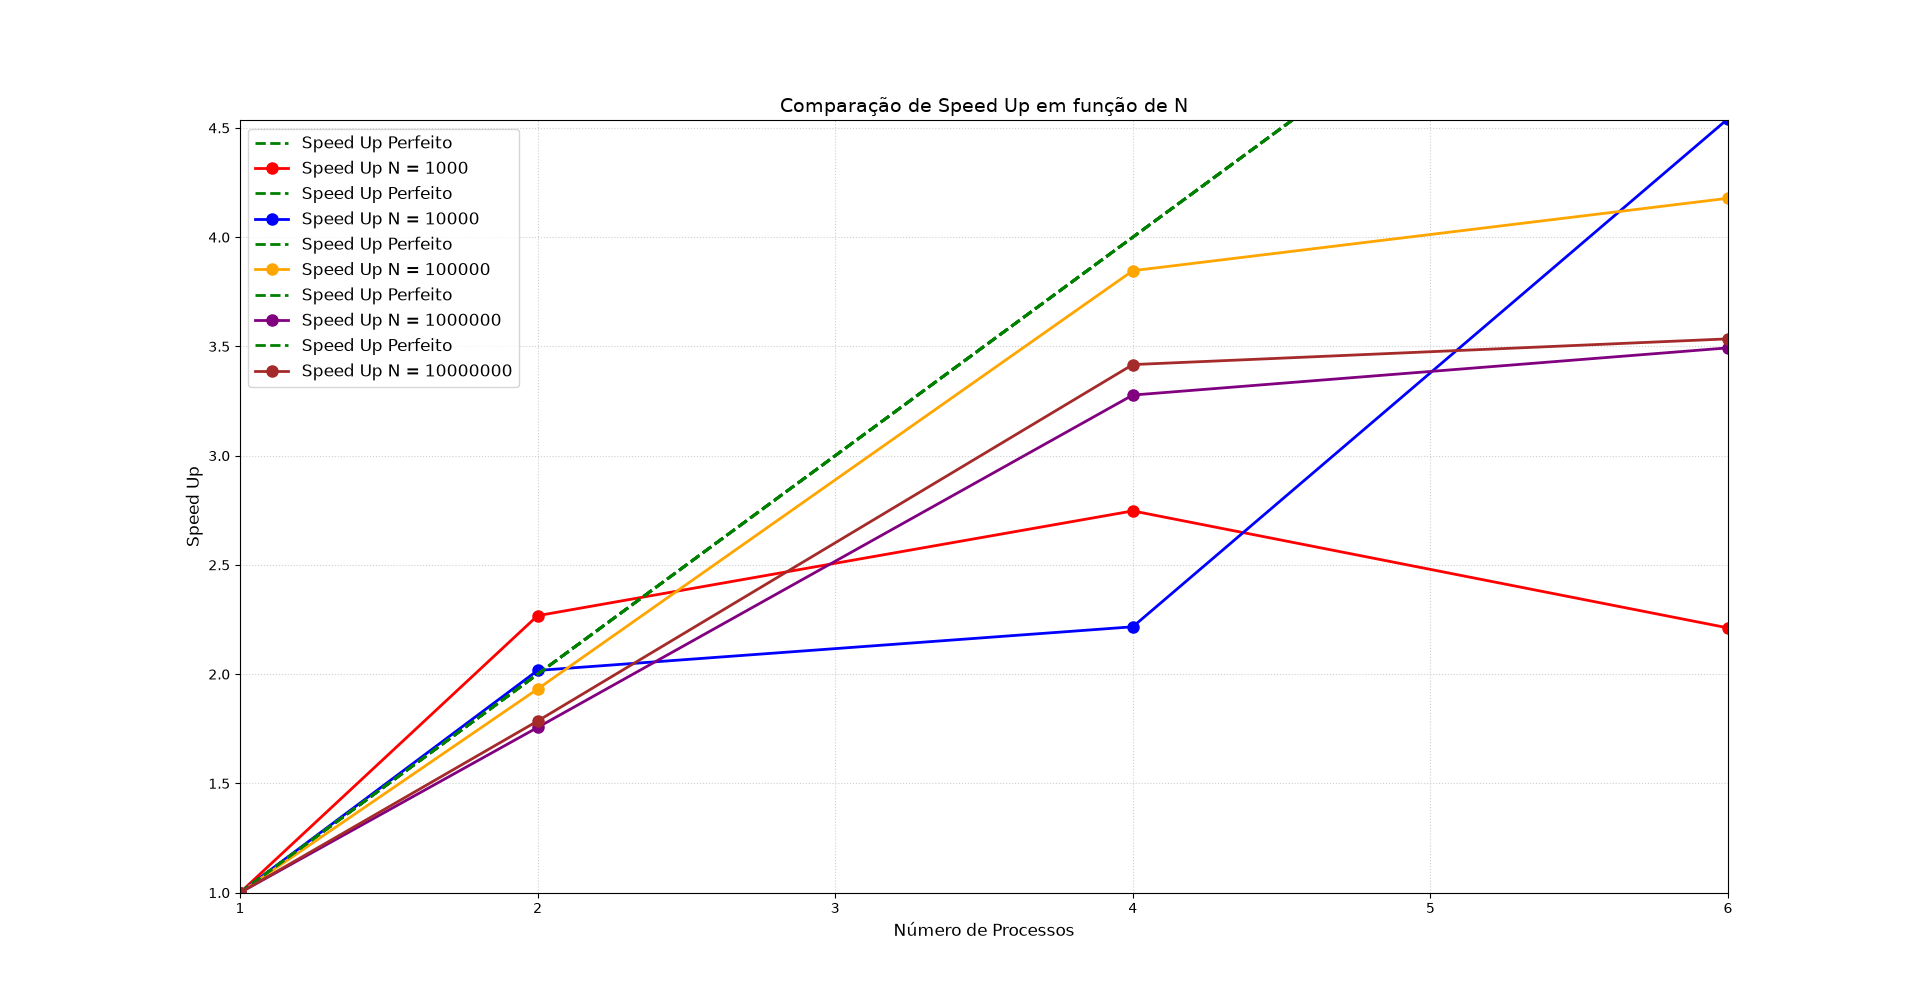
\includegraphics[width=1.2\textwidth]{figuras/primos_speed_up.png}
    \caption{SpeedUp para diferentes valores de N e número de processos.}
    \label{fig:primos_efficiency}
\end{figure}

\begin{figure}[H]
    \centering
    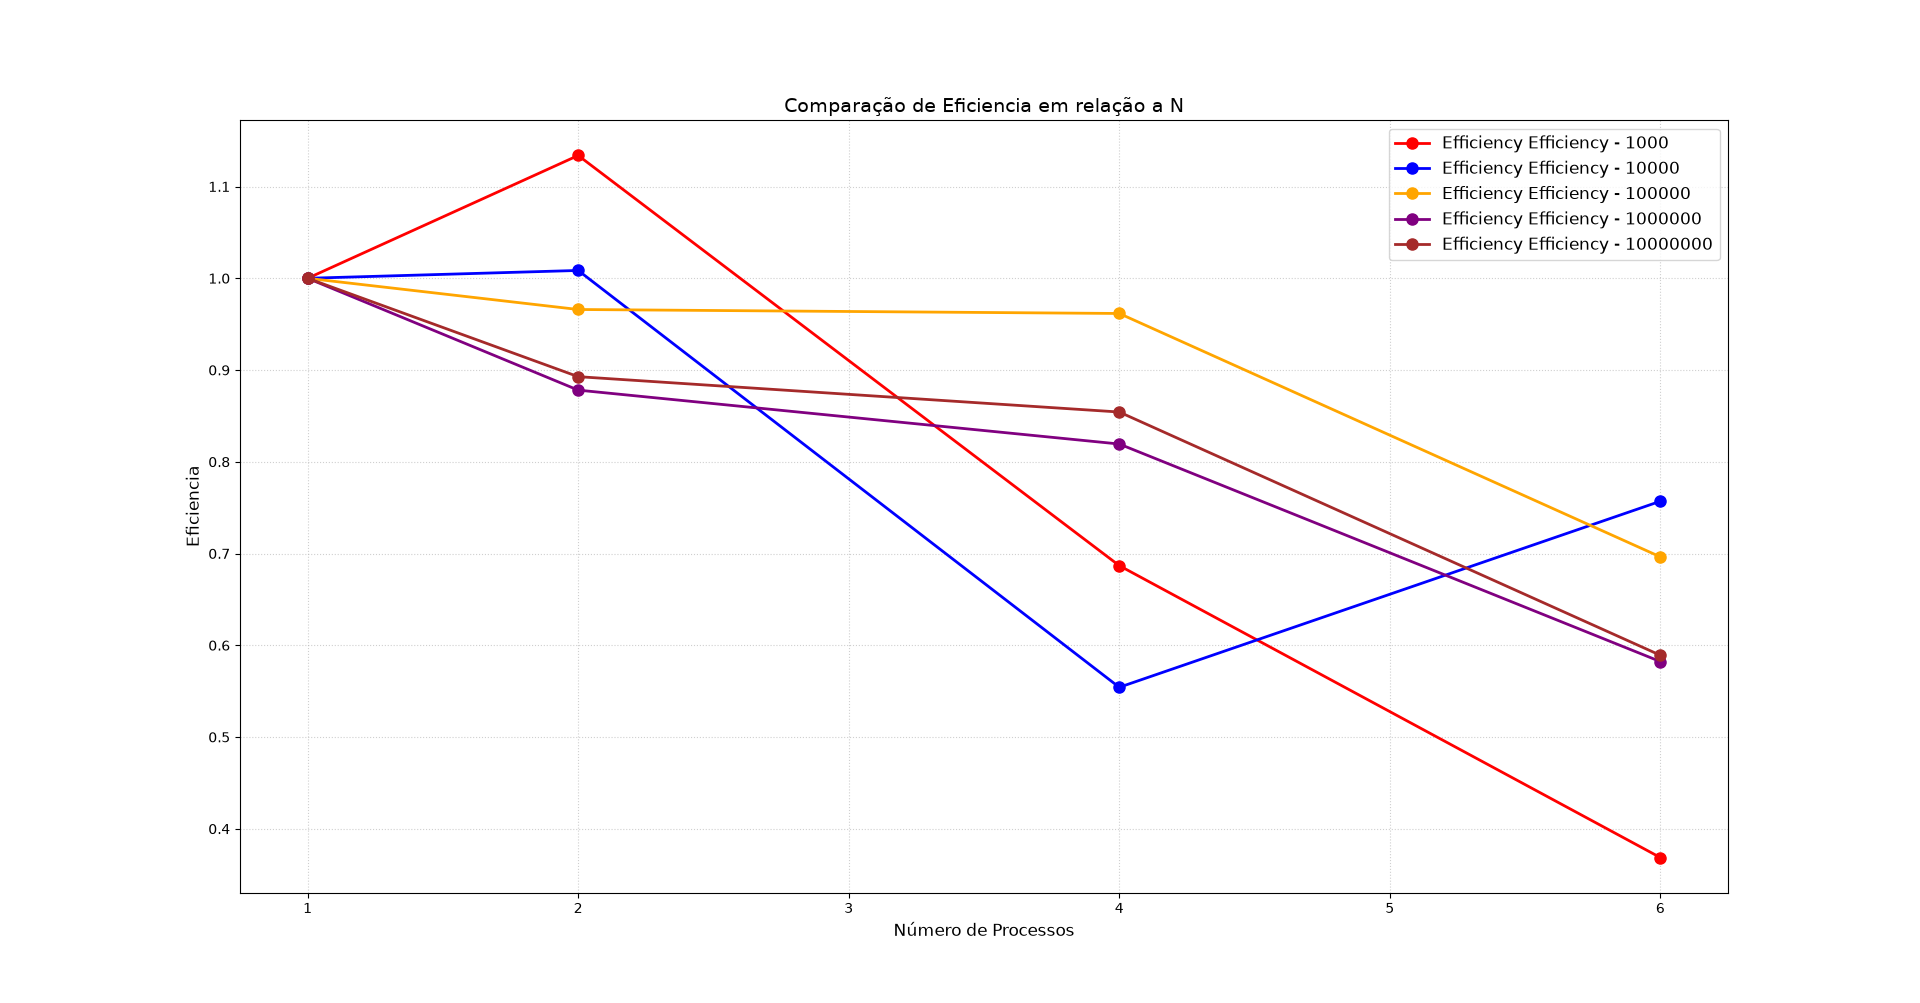
\includegraphics[width=1.2\textwidth]{figuras/primos_efficiency.png}
    \caption{Eficiência para diferentes valores de N e número de processos.}
    \label{fig:primos_efficiency}
\end{figure}


Quanto maior o número de números a serem testados, maior o tempo de execução, pois quanto maior o número a ser testado, mais tempo ele leva para ser testado. A distribuição foi feita de forma cíclica, ou seja, a distribuição está homogênea, logo nenhum processo está sobrecarregado. 

Para a fase de broadcast e scater, como os elementos são alocados localmente, o custo de comunicação é irrelevante, visto que o único elemento compartilhado é o número total de números a serem testados(não o vetor contendo esses números). 

Para a fase de gather, o custo representa a necessidade de cada processo enviar a lista com os números primos por ele encontrados, como a divisão é homogênea, em tese essa lista tem tamanho similar, logo o custo de comunicação deve ser mais ou menos constante.

Cada processo é criado uma única vez e eles devem apenas retornar a lista de números primos, que pode ser obtida com um gather e não há necessidade de sincronização, visto que cada processo é independente e não há necessidade de esperar por outros processos, pois eles só buscam por primos dentro do intervalo que lhes foi atribuído.

Observando as curvas, nota-se que a partir de N = 100 000 o speed up apresenta um comportamento semelhante para os demais valores de N, onde até 4 processos o crescimento é quase igual ao perfeito, mas para o processo 6 ele começa a cair. A eficiência também cai de forma quase que constante. Por conta desse comportamento semelhante, conclui-se que a partir de N = 100 000 começa a valer a pena paralelizar com pelo menos 4 processos.


% ---
% Finaliza a parte no bookmark do PDF, para que se inicie o bookmark na raiz
% ---
\bookmarksetup{startatroot}% 
% ---

% ----------------------------------------------------------
% ELEMENTOS PÓS-TEXTUAIS
% ----------------------------------------------------------
\postextual

% ----------------------------------------------------------
% Referências bibliográficas
% ----------------------------------------------------------
\bibliography{references}
\clearpage

% ----------------------------------------------------------
% Glossário
% ----------------------------------------------------------
%
% Há diversas soluções prontas para glossário em LaTeX. 
% Consulte o manual do abnTeX2 para obter sugestões.
%
%\glossary

% ----------------------------------------------------------
% Apêndices
% ----------------------------------------------------------

% ---
% Inicia os apêndices
% ---
\begin{apendicesenv}

% ----------------------------------------------------------
\chapter{Encontrar Primos dentro do intervalo N} \label{app:code}

\lstinputlisting[language=Python, caption={Encontrar Primos dentro do intervalo N}, label={app:primos}]{appendices/encontrar\_primos.py}
% ----------------------------------------------------------

\end{apendicesenv}
% ---

% ----------------------------------------------------------
% Anexos
% ----------------------------------------------------------
\cftinserthook{toc}{AAA}
% ---
% Inicia os anexos
% ---
%\anexos
\begin{anexosenv}

% ---
% ---

\end{anexosenv}

\end{document}
